\documentclass[a4paper]{report}
\usepackage[T1]{fontenc} % Fontes T1
\usepackage[utf8]{inputenc} % Input UTF8
\usepackage[backend=biber, style=ieee]{biblatex} % para usar bibliografia
\usepackage{csquotes}
\usepackage[portuguese]{babel} %Usar língua portuguesa
\usepackage{blindtext} % Gerar texto automaticamente
\usepackage[printonlyused]{acronym}
\usepackage{hyperref} % para autoref
\usepackage{graphicx}
\usepackage{float}
\usepackage{amsmath, amsfonts, amssymb}
\usepackage{caption}

\bibliography{bibliografia.bib}


\begin{document}
%%
% Definições
%
\def\titulo{Cliente para acesso a sonda}
\def\data{20 de Abril de 2018}
\def\autores{Ricardo Ermida, Rodrigo Santos}
\def\autorescontactos{(89187) ricardoermida@ua.pt, (89180) rodrigo.l.silva.santos@ua.pt}
\def\versao{1.0}
\def\departamento{DETI - Universidade de Aveiro}
\def\empresa{Universidade de Aveiro}
\def\logotipo{ua.pdf}
%
%%%%%% CAPA %%%%%%
%
\begin{titlepage}

\begin{center}
%
\vspace*{50mm}
%
{\Huge \titulo}\\ 
%
\vspace{10mm}
%
{\Large \empresa}\\
%
\vspace{10mm}
%
{\LARGE \autores}\\ 
%
\vspace{30mm}
%
\begin{figure}[h]
\center
\includegraphics{\logotipo}
\end{figure}
%
\vspace{30mm}
\end{center}
%
\begin{flushright}
\versao
\end{flushright}
\end{titlepage}

%%  Página de Título %%
\title{%
{\Huge\textbf{\titulo}}\\
{\Large \departamento\\ \empresa}
}
%
\author{%
    \autores \\
    \autorescontactos
}
%
\date{\data}
%
\maketitle

\pagenumbering{roman}

%%%%%% RESUMO %%%%%%
\begin{abstract}
Os monitores de computadores são a principal unidade de saída dos computadores, uma unidade de muita importância uma vez que é atravez dela que conseguimos ver e analisar o que estamos a fazer num computador. Os monitores, tal como todos os outros aparelhos eletrónicos de grande importância, têm vindo a ser alvo de grande evolução. Começando por ser dispositivos que comunicavam com o utilizador atravéz de luzes que se acendiam e apagavam em determinadas posições em função das intruções que executavam, evoluindo depois para monitores capazes de apresentar algumas cores e com resoluções já consideráveis, até se desenvolverem os monitores que hoje são utilizados na grande maioria dos computadores que já são capazes de exibir milhões de cores e pussuem resoluções de exibição muito maiores que os anteriores.
Um pixel é o menor elemento numa unidade de exibição como por exemplo o monitor, ao qual se pode atribuir uma cor. Cada pixel tem 3 subpíxeis um de cor vermelha outro azul e outro verde e dependendo do brilho de cada um, o pixel adquire uma cor. A sua organização num monitor afeta muito a qualidade de imagem do monitor e isso é visivél na comparação de imagens em monitores com organizações diferentes.
A resolução de um monitor é apenas o número de píxeis capazes de ser exibidos horizontalmente e verticalmente num monitor, podendo por esse motivo ser um termo ambíguo e que não nos diz nada acerca da qualidade de imagem do monitor. 

\end{abstract}

%%%%%% Agradecimentos %%%%%%
% Segundo glisc deveria aparecer após conclusão...
\renewcommand{\abstractname}{Agradecimentos}
\begin{abstract}
Gostaríamos de agradecer ao nosso professor de Laboratórios de Informática pela liberdade de escolha do tema deste relatório, tornando esta tarefa mais agradavél e motivadora, e também pela tentativa de resolução de alguns problemas que encontrámos na elaboração do relatório.
\end{abstract}


\tableofcontents
% \listoftables     % descomentar se necessário
% \listoffigures    % descomentar se necessário


%%%%%%%%%%%%%%%%%%%%%%%%%%%%%%%
\clearpage
\pagenumbering{arabic}

%%%%%%%%%%%%%%%%%%%%%%%%%%%%%%%%
\chapter{Introdução}
\label{chap.introducao}

O tema que iremos abordar neste relatório será "Monitores", um tema de muito interesse para os membros deste grupo; como estudantes matriculados no curso de \ac{miect}; uma vez que os monitores são hoje em dia indispensáveis para facilitar o trabalho de muitos trabalhadores.

Será feito um aprofundamento acerca de todos os aspectos mais importantes de um monitor com o intuíto de se perceber como estes funcionam, e qual a sua evolução ao longo do tempo.

Este relatório está dividido em 5 capítulos.

Depois desta introdução, no \autoref{chap.História} é apresentada um pouco da história dos monitores, este capítulo encontra-se dividido em 3 subcapítulos no primeiro é explicado o que é um \ac{crt}, no segundo o que é um \ac{lcd} por fim no terceiro analisaremos as vantagens e desvantagens de ambos. No \autoref{chap.Cores} iremos abordar o tópico das cores num monitor, abordando o que é, como funcionam os píxeis e como a partir daí são criadas as cores, seguidamente no \autoref{chap.Resolução} iremos explicar o que é a resolução bem como a sua importância num monitor. Por fim, no \autoref{chap.conclusao} são apresentadas as conclusões retiradas após terminado o trabalho.

\chapter{História}
\label{chap.História}

Os ecrãs ou monitores de um computador são o seu principal dispositivo de saída (output), podendo, contudo, também ser uma unidade de entrada/saída (input/output) se este pussuir uma tela touch ou multitátil.

Os primeiros computadores comunicavam a partir de pequenas luzes, que se acendiam ou se apagavam ao aceder a determinadas posições de cor ou a executar certas instruções. Anos mais tarde apareceram computadores que funcionavam com cartão perfurado, que permitiam introduzir programas no computador. E só na década de 70 surgiram os primeiros monitores \ac{crt} estes seguiam o \ac{mda}, e eram monitores monocromáticos que exibiam uma única cor, o verde. Ainda no mesmo ano saíram os monitores \ac{cga}, estes foram comercializados em 1981 e com eles desenvolveu-se a primeira placa de vídeo colorida da \ac{ibm}. Ambos os monitores entraram no mercado ao mesmo tempo mas os monitores monocromáticos tiveram mais vendas que os monitores \ac{cga} porque o custo era mais acessível para os utentes.Três anos mais tarde surgiu o monitor \ac{ega} desenvolvido pela \ac{ibm} para a visualização de gráficos, este monitor contribuía mais cores (16) e uma maior resolução.(\cite{mc})\\
\begin{center}
\begin{figure}[H]
\center
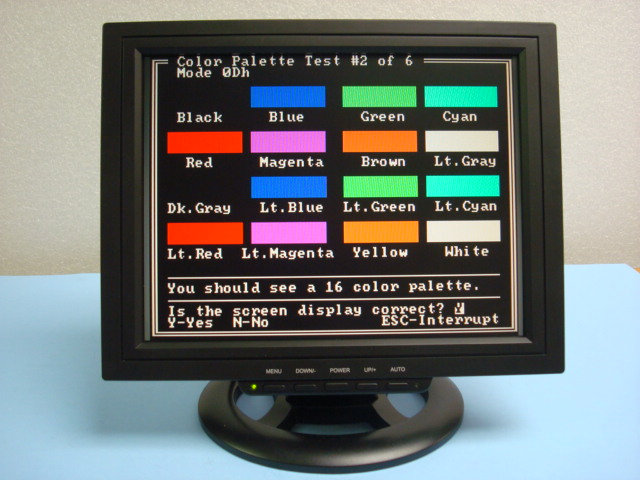
\includegraphics[width=3cm]{imagens/cga.JPG}
\caption{Monitor \ac{ega}}
\end{figure}
\end{center}
Em 1987 apareceu o \ac{vga} foi um monitor que teve muito sucesso no mercado e dois anos mais tarde foi melhorado e redesenhado para solucionar certos problemas que surgiram, desenvolvendo assim o \ac{svga}, que também aumentava as cores e as resoluções, para este novo monitor  desenvolveram-se placas de vídeo de fabricantes que ainda hoje são conhecidos, tais como S3 Graphics, NVIDIA ou ATI entre outros.(\cite{mc})
\begin{center}
\begin{figure}[h]
\center
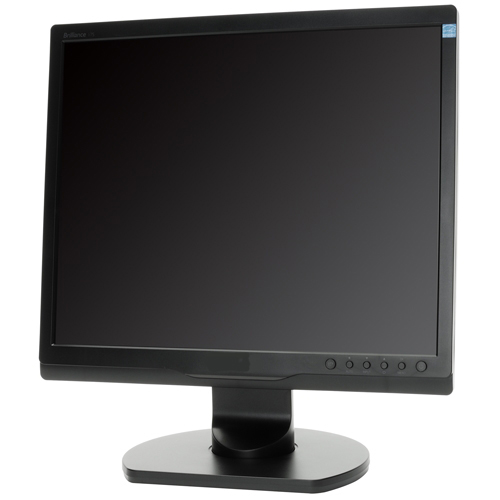
\includegraphics[width=2.5cm]{imagens/vga.jpg}
\caption{Monitor \ac{vga}}
\end{figure}
\end{center}
Foi também nos anos 80 que começaram a nascer os monitores \ac{lcd} mas estes não foram muito bem acolhidos na altura, devido a serem muito caros e a terem a mesma eficiência que um monitor comum, sendo só usados em notebooks.(\cite{mc})

\section{Monitores CRT}
Um monitor \ac{crt} é um monitor que utiliza um tubo de raios catódicos para criar imagens.
Um tubo de raios catódicos é um tipo de válvula eletrónica que contem um ou mais canhões de eletrões e um ecrã fluorescente utilizado para ver imagens. (\cite{crt})
\begin{center}
\begin{figure}[h]
\center
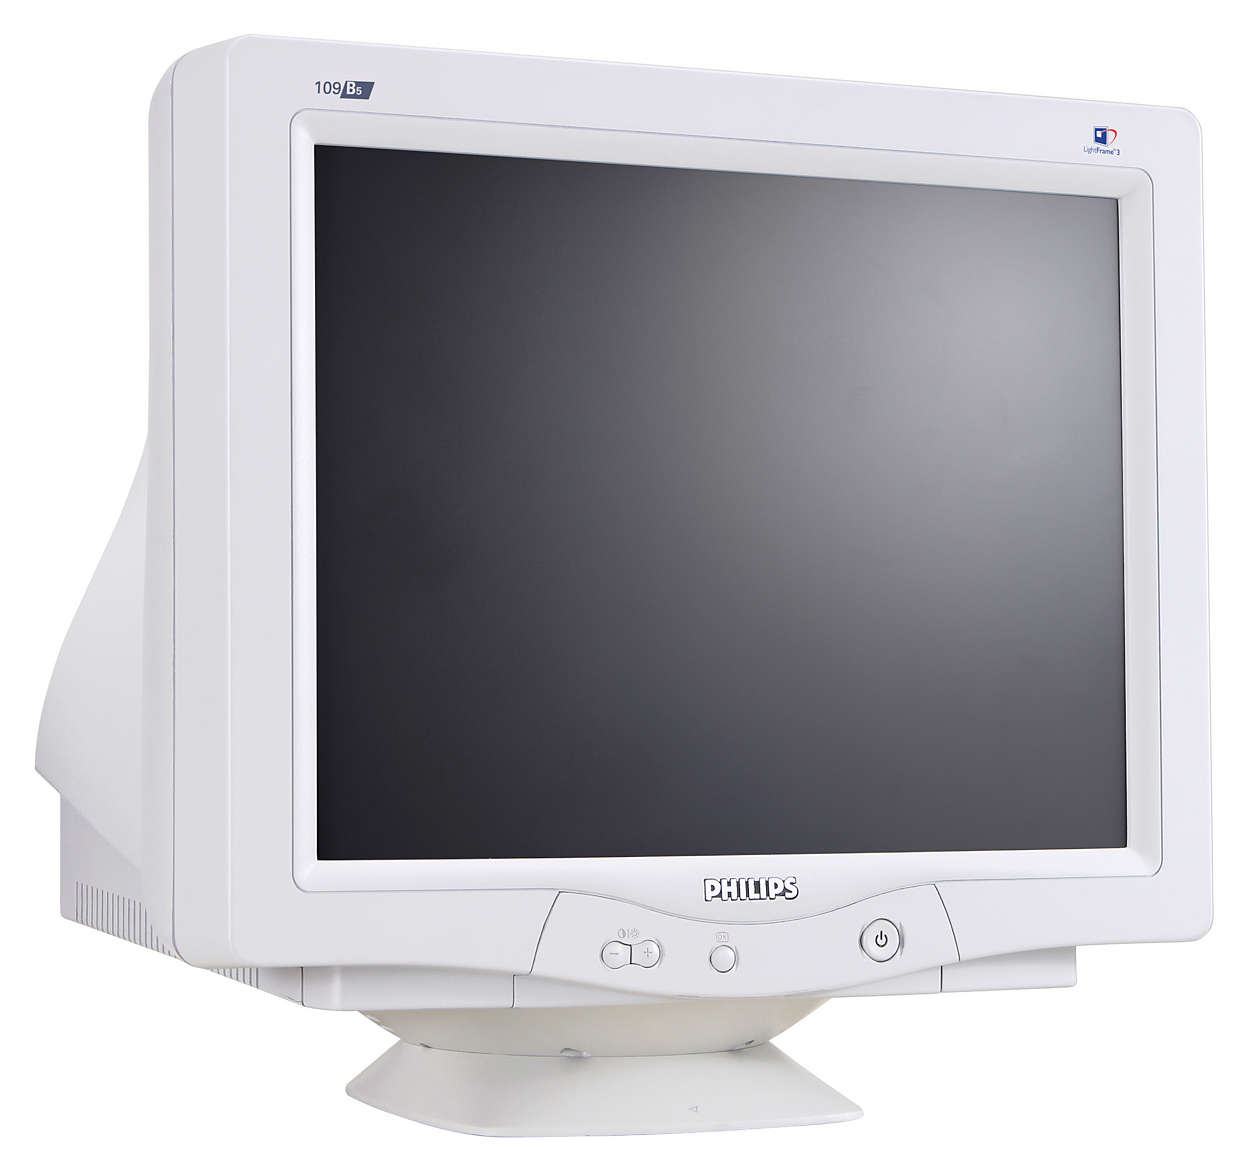
\includegraphics[width=2.5cm]{imagens/crt.jpeg}
\caption{Monitor \ac{crt}}
\end{figure}
\end{center}

\section{Monitores LCD}

Um \ac{lcd} é um painel fino usado para exibir informações por via eletrônica, como texto, imagens e vídeos. O seu uso inclui monitores para computadores, televisores, painéis de instrumentos e outros dispositivos, que vão desde cockpit de aeronaves, displays em computadores de bordo de automóveis, a dispositivos de utilização diárias, tais como leitores de vídeo, dispositivos de jogos, relógios, calculadoras e telefones. (\cite{lcd})
\begin{center}
\begin{figure}[h]
\center
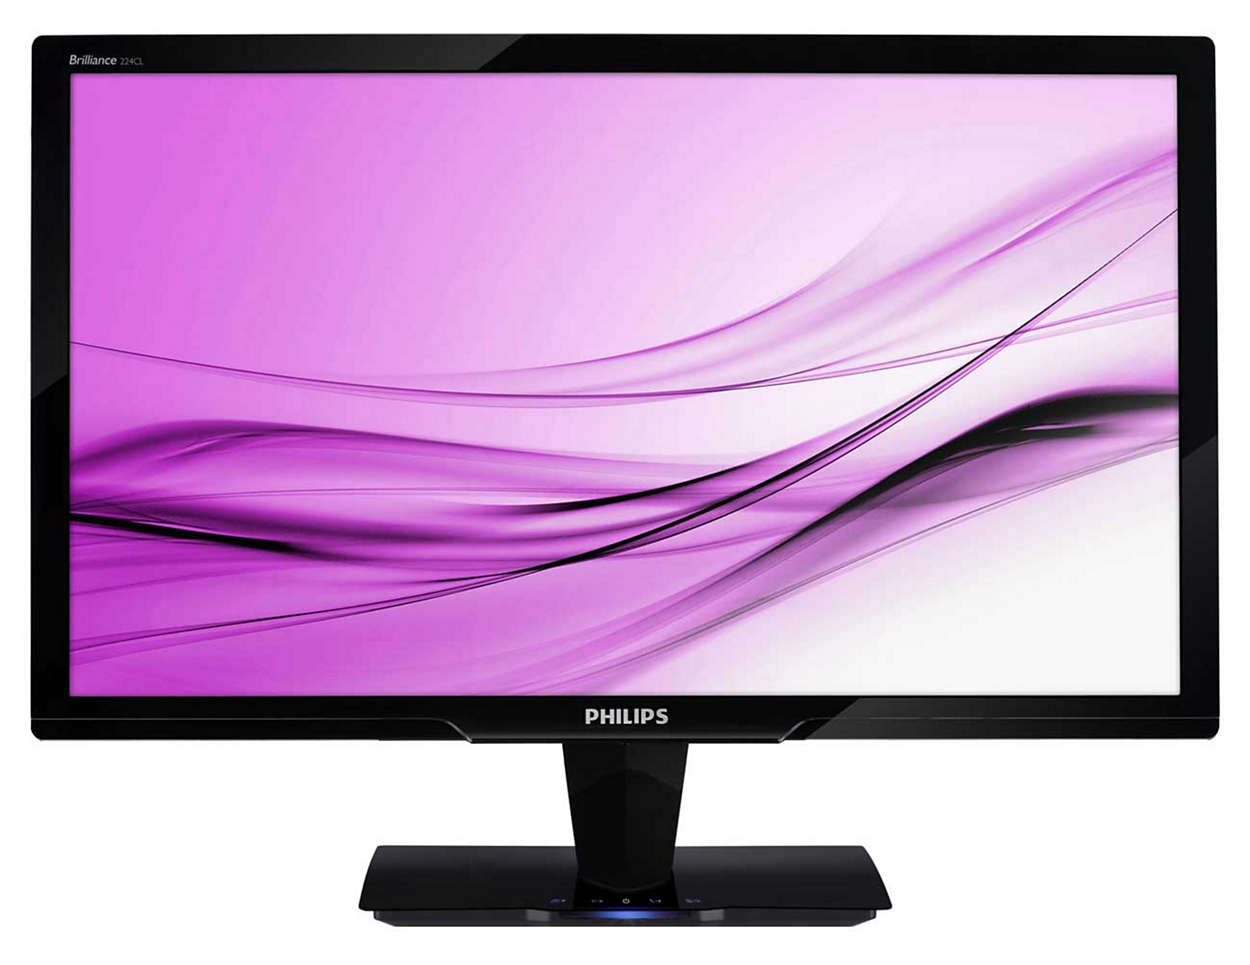
\includegraphics[width=2.5cm]{imagens/lcd.jpeg}
\caption{Monitor \ac{lcd}}
\end{figure}
\end{center}

\section{Monitores CRT vs Monitores LCD}
Nesta secção iremos abordar algumas das vantagens e das desvantagens dos monitores CRT e LCD.\\
Vantagens e desvantagens dos monitores CRT. (\cite{mv})
\begin{itemize}
	\item Vantagens:
		\begin{enumerate}
		\item longa vida útil.
		\item baixo custo de fabrico.
		\item  pode funcionar em diversas resoluções, sem que ocorram grandes distorções na imagem.
		\end{enumerate}
\end{itemize}
\begin{itemize}
	\item Desvantagens:
		\begin{enumerate}
		\item dimensões muito grandes.
		\item elevado consumo de energia.
		\item a possibilidade de emitir radiação perigosa para a saúde do ser humano  no caso de longos períodos de exposição.
		\end{enumerate}
\end{itemize}
Vantagens e desvantagens dos monitores LCD.
\begin{itemize}
	\item Vantagens:
		\begin{enumerate}
		\item O baixo consumo de energia.
		\item As dimensões e peso são reduzidas.
		\item A capacidade de formar uma imagem praticamente perfeita, estável, que cansa menos a visão.
		\end{enumerate}
\end{itemize}
\begin{itemize}
	\item Desvantagens:
		\begin{enumerate}
		\item grande custo de fabricação.
		\item ao trabalhar numa resolução diferente daquela para a qual foi projetado, utiliza vários artifícios de composição de imagem que acabam por degradar a qualidade final da mesma.
		\item se o cristal líquido da tela do monitor for danificado e ficar exposto ao ar, pode emitir alguns compostos tóxicos.
		\end{enumerate}
\end{itemize}


\chapter{Cores}
\label{chap.Cores}

Um pixel é o menor elemento num dispositivo de exibição (por exemplo, um monitor), ao qual é possível atribuir-se uma cor. De uma forma mais simples, um pixel é o menor ponto que forma uma imagem digital, sendo que o conjunto de píxeis formam a imagem inteira.
Cada pixel tem interiormente 3 subpíxeis, um vermelho, um verde e outro azul; dependendo do brilho da cada um dos subpíxeis, o pixel adquire uma cor de forma semelhante à composição de cores RGB. \ac{rgb} é a abreviatura do sistema de cores aditivas formado por Vermelho (Red), Verde (Green) e Azul (Blue). O propósito principal do sistema \ac{rgb} é a reprodução de cores em dispositivos eletrónicos como monitores de televisão e computador, retroprojetores, scanners e câmaras digitais, assim como na fotografia tradicional.
Uma pergunta que se surge bastante quando se fala sobre o tópicos das cores num monitor é: como se deve organizar os subpíxeis de um monitor? Costumam-se organizar em linhas verticais, mas para melhorar a sensação de movimento, é melhor organizá-los em diagonal ou em triângulos. O conhecimento do tipo de organização de píxeis, pode ser utilizado para melhorar a visualização de imagens de mapas de bits, um mapa de bit são imagens que contêm a descrição de cada pixel.
Outro termo que é muito utilizado no que toca a cores num monitor é a profundidade de cor, a maior parte dos monitores têm uma profundidade de 8 bits por cor (24 bits ao todo), isto é, podem representar aproximadamente 16,8 milhões de cores diferentes.
A profundidade de cor é um termo da computação gráfica que descreve a quantidade de bits usados para representar a cor de um único pixel numa imagem bitmap. Este conceito é conhecido também como bits por pixel (bpp), particularmente quando especificado junto com o número de bits usados. Quanto maior a quantidade da profundidade da cor presente na imagem, maior é a escala de cores disponível.
Como podemos verificar pela comparação entre as próximas duas imagens, os subpíxeis do monitor \ac{lcd} estão muito melhor organizados que os subpíxeis do monitor \ac{crt}. (\cite{p, mc, mb, pc})
\begin{center}
\begin{figure}[H]
\center
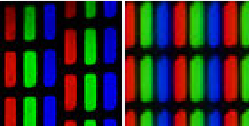
\includegraphics[width=3.25cm]{imagens/crtp.png}
\caption{Disposição dos subpíxeis \ac{crt} à esquerda e \ac{lcd} à direita (\cite{mc})}
\end{figure}
\end{center}
Na imagem seguinte podemos observar o impacto que a organização dos subpíxeis tem na qualidade das cores das imagens de ambos os monitores(quanto melhor for a organização dos subpíxeis melhor será a qualidade das cores das imagens).
\begin{center}
\begin{figure}[H]
\center
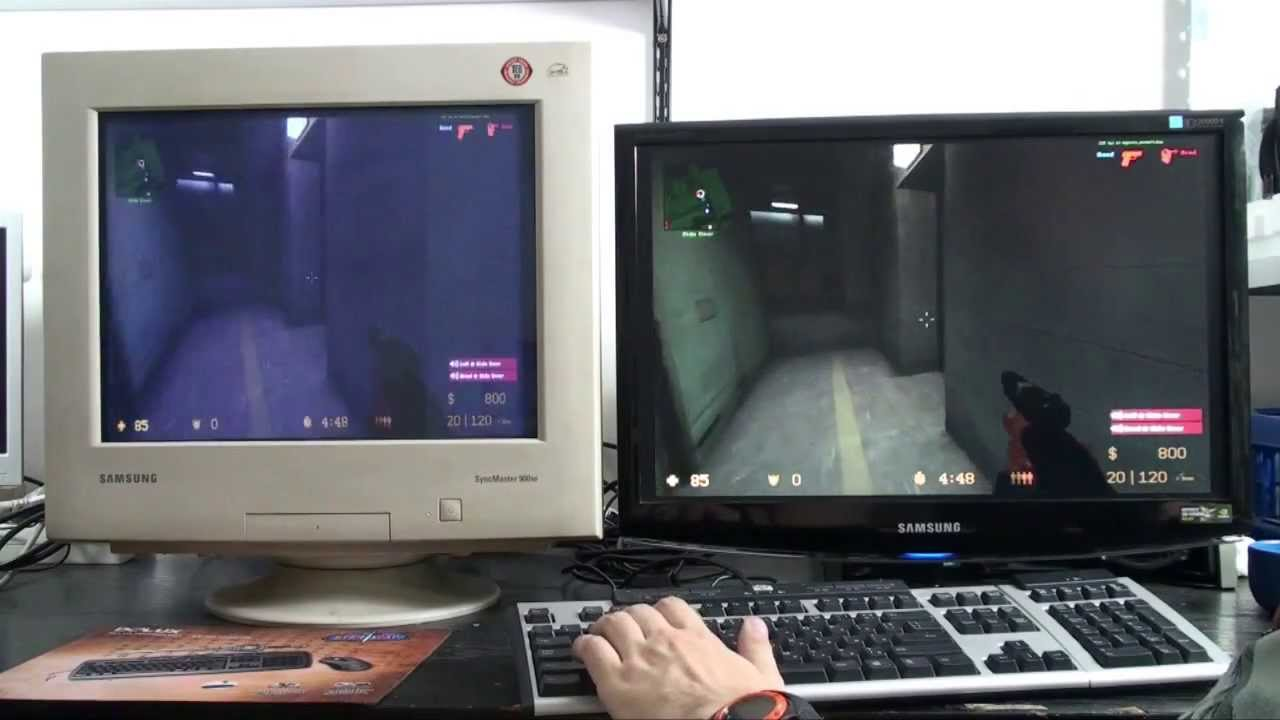
\includegraphics[width=8.5cm]{imagens/comp.jpg}
\caption{Imagem em monitor \ac{crt} à esquerda e \ac{lcd} à direita}
\end{figure}
\end{center}

\chapter{Resolução}
\label{chap.Resolução}

Outro fator também muito importante nos monitores atuais é a sua resolução. Sendo esta o número máximo de píxeis capazes de serem mostrados em cada dimensão do monitor, isto é horizontalmente e verticalmente. Quando nos referimos á resolução, normalmente referimos da forma \textbf{\texttt{largura/altura}}, e utilizando como unidade o pixel, por exemplo quando mencionamos uma resolução do tipo "1920x1080" isto significa que a largura é de 1920 píxeis e a altura é de 1080 píxeis, originando também 1920 linhas de píxeis e 1080 colunas de píxeis, o que perfaz um total de 2,073,600 píxeis para um monitor com uma resolução deste tipo.\\ No entanto é um termo ambíguo especialmente porque a resolução mostrada é controlada por diferentes fatores dependendo do tipo de monitor em causa.\\ Monitores do tipo \ac{lcd}, \ac{pdp}, \ac{dlp}, entre outros similares exibem um número fixo de píxeis (fixed-pixel-array displays),ou seja pussuem uma única resolução nativa possível, nestes casos o uso do termo resolução refere-se simplesmente ao número de colunas e linhas de píxeis que criam a imagem mostrada no monitor. Uma das desvantagens deste tipo de monitores é que todos eles precisam de um sistema de escalonamento; um processador de video digital que contem um array de memória; para fazer corresponder uma imagem ou video com formato diferente ao do monitor para que este seja então exibido. O que pode gerar artefactos nas imagens se o monitor for forçado a trabalhar numa resolução não nativa.\\
A tabela abaixo apresenta os tipos de resolução mais utilizados atualmente.(\cite{dr})
\begin{center}
\begin{tabular}{c|c|c|c|c}\\

Padrão & Largura (px.) & Altura (px.) & \% Utilizadores \\ \hline

HD & 1366 & 768 & 29.94\\ 

FHD & 1920 & 1080 & 16.02\\

WXGA+ & 1440 & 900 & 6.70\\

HD+ & 1600 & 900 & 5.89\\ 

\end{tabular}
\end{center}

\begin{itemize}
	\item \textbf{HD} - High Definition
	\item \textbf{FHD} - Full High Definition
	\item \textbf{WXGA+} - Widescreen Extended Graphics Array Plus
	\item \textbf{HD+} - High Definition plus
\end{itemize}
Dois monitores com a mesma resolução podem ter dimensões diferentes dependendo mais uma vez do tipo de monitor em causa, se este for \ac{lcd} uma dimensão de 17 polegadas (unidade de medida utilizada para determinar o tamanho de dispositivos de exibição, que é a distância entre um canto superior do monitor ao canto inferior oposto) terá a mesma zona visivel de um monitor \ac{crt} com uma dimensão de 19 polegadas.
A proporção da tela é um fator relacionado com a resolução de um monitor, uma vez que é a relação entre o número de píxeis existentes em cada coluna de píxeis e o número de píxeis existentes em cada linha de píxeis do monitor. A proporção está por sua vez relacionada com o padrão de exibição. (\cite{mc, gdr})

A figura a seguir contém os diferentes tipos de resoluções e proporções de tela e associa-os aos diferentes padrões de exibição existentes.

\begin{center}
\begin{figure}[h]
\center
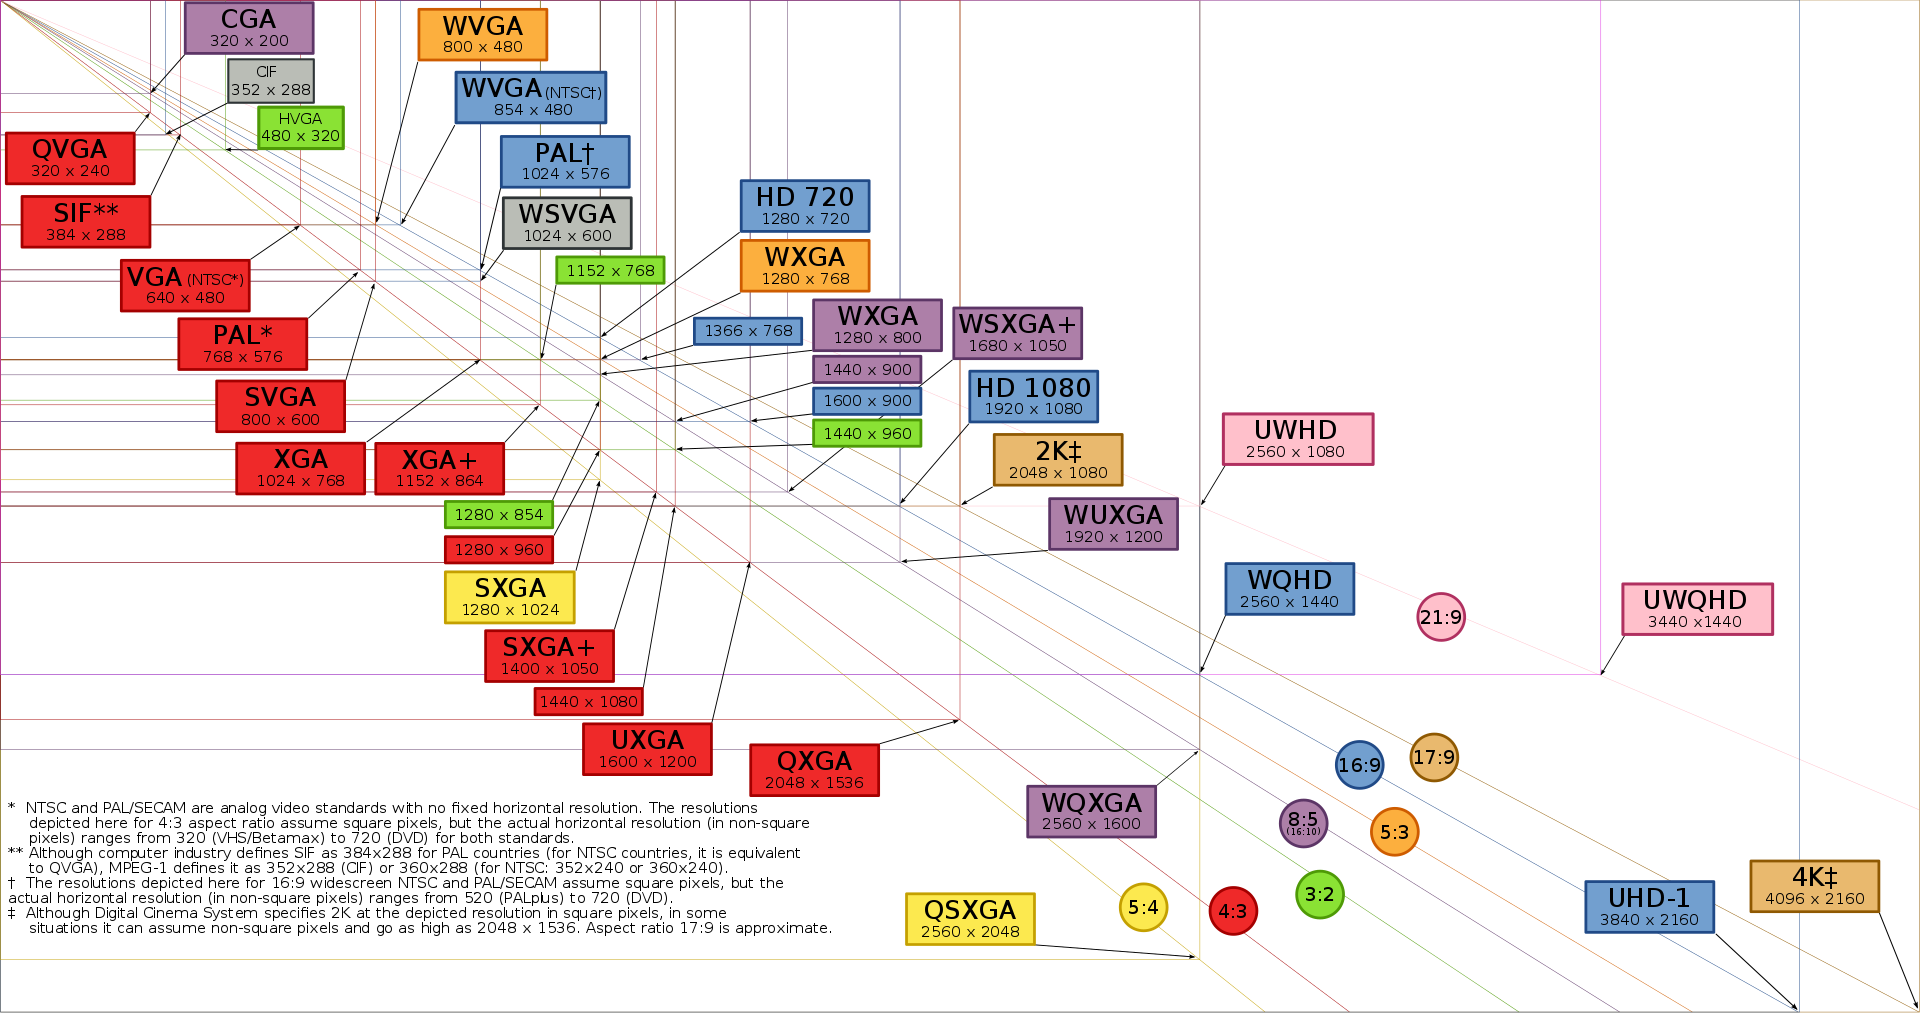
\includegraphics[width=12cm]{imagens/padroes.png}
\caption{Relação entre padrões, resoluções e proporções (\cite{dr})}
\end{figure}
\end{center}

\chapter{Conclusões}
\label{chap.conclusao}

Em suma os monitores são hoje em dia algo indispensável e de extrema importância, uma vez que tal como as nossas mentes não nos seriam muito úteis se não conseguissemos por em prática e partilhar os nossos pensamentos e ideias, um computador também não se não soubessemos ou não nos fosse mostrado o que nele estavamos a operar. Daí também a constante procura e desenvolvimento de maneiras de tornar os monitores cada vez mais capazes em todos os seus aspetos desde a resolução ao tipo de píxeis utilizados para que possamos disfrutar de resoluções cada vez maiores e qualidades de imagem cada vez melhores, tornando assim o trabalho diário de milhares de pessoas nos computadores mais apelativo.
Foi provado no relatório que os dois tipos de monitores mais utilizados hoje em dia pussuem as suas vantagens e desvantagens, que a qualidade de imagem de um monitor não está apenas relacionada com a sua resolução mas também com a disposição dos píxeis e subpíxeis num monitor.

\chapter*{Contribuições dos autores}

No desenvolvimento deste relatório ambos os membros do grupo demonstraram o empenho necessário para a sua conclusão.
O Ricardo Ermida desenvolveu o capítulo da história e das cores, tendo o Rodrigo Santos feito o capítulo da Resolução, a introdução e o resumo. Ambos releram o relatório várias vezes para certificar de que não havia erros de qualquer espécie e para que fosse alterado, se necessário, algum do conteúdo, a conclusão bem como a inserção de acrónimos foi realizada por ambos os membros.
Assim o trabalho desenvolvido pelo RS e pelo RE foi de 50\% cada um.


%%%%%%%%%%%%%%%%%%%%%%%%%%%%%%%%%
\chapter*{Acrónimos}
\begin{acronym}
\acro{ua}[UA]{Universidade de Aveiro}
\acro{miect}[MIECT]{Mestrado Integrado em Engenharia de Computadores e Telemática}
\acro{crt}[CRT]{Cathode Ray Tube}
\acro{lcd}[LCD]{Liquid-Crystal Display}
\acro{rgb}[RGB]{Red Green and Blue}
\acro{mda}[MDA]{Monocromatic Display Adapter}
\acro{cga}[CGA]{Color Graphics Adapter}
\acro{ibm}[IBM]{International Business Machines}
\acro{ega}[EGA]{Enhanced Graphics Adapter}
\acro{vga}[VGA]{Video Graphics Array}
\acro{svga}[SVGA]{Super VGA}
\acro{pdp}[PDP]{Plasma Display Panels}
\acro{dlp}[DLP]{Digital Light Processing}
\end{acronym}

\chapter*{Bibliografia}
*NOTA: Nenhuma da informação deste relatório é da nossa autoria. Foi toda retirada dos seguintes sites:\\

\textit{Display resolution}, 
\url{https://en.wikipedia.org/wiki/Display_resolution},
Acedido a: 2017-11-15.\\

\textit{Monitor de computador}, 
\url{https://pt.wikipedia.org/wiki/Monitor_de_computador#Hist.C3.B3ria},
Acedido a: 2017-11-14.\\

\textit{LCD}, 
\url{https://pt.wikipedia.org/wiki/LCD#Hist.C3.B3ria},
Acedido a: 2017-11-15.\\

\textit{Monitor de vídeo}, 
\url{https://pt.wikipedia.org/wiki/Monitor_de_v\%C3\%ADdeo},
Acedido a: 2017-11-15.\\

\textit{Graphics display resolution}, 
\url{https://en.wikipedia.org/wiki/Graphics_display_resolution#WSXGA.2B_.281680.C3.971050.29}, \\Acedido a: 2017-11-16.\\

\textit{CRT}, 
\url{https://pt.wikipedia.org/wiki/Tubo_de_raios_cat\%C3\%B3dicos}, \\Acedido a: 2017-11-15.\\

\textit{Raster}, 
\url{https://pt.wikipedia.org/wiki/Raster}, Acedido a: 2017-11-15.\\

\textit{Pixel}, 
\url{https://pt.wikipedia.org/wiki/Pixel}, Acedido a: 2017-11-15.\\

\textit{Profundidade de cor}, 
\url{https://pt.wikipedia.org/wiki/Profundidade_de_cor}, Acedido a: 2017-11-15.\\

%%%%%%%%%%%%%%%%%%%%%%%%%%%%%%%%%
\printbibliography

\end{document}
